\part{Cifrari simmetrici moderni}
\chapter{\emph{Data Encryption Standard} (DES)}
\section{Introduzione e principi di Shannon}
Il \emph{Data Encryption Standard} è un cifrario simmetrico che è stato lo standard per la crittografia di massa fino all'avvento dell'AES Pur non essendo più usato è importante conoscerlo: i cifrari moderni si basano sulla struttura del DES. Il DES è il primo algoritmo a basarsi sui principi di Shannon.
\begin{itemize}
    \item \textbf{Diffusione}: ogni singolo carattere del crittogramma dipende da \underline{\textbf{tutti}} i caratteri del testo in chiaro.
    \item \textbf{Confusione}: combinare testo in chiaro e chiave in modo complesso in modo che osservare il crittogramma non possa portare a separare le due sequenze (testo in chiaro e chiave).
\end{itemize}
Questi principi sono importanti per la resistenza agli attacchi di crittoanalisi statistica.

\section{Storia}
Nasce nel 1972 quando NBS (\textit{National Bureau of Standard}) ora NIST (\textit{National Institute for Security and Technology}) chiese la creazione di un algoritmo di crittografia simmetrica standard (standard poichè ogni compagnia usava un proprio sistema crittografico). 
\paragraph{Richieste dell'ente} In particolare le richieste erano:
\begin{itemize}
    \item sicurezza basata sulla segretezza della chiave e non sul processo di cifratura e decifrazione (tutto pubblico tranne la chiave);
    \item l'algoritmo doveva essere efficiente sia in software che in hardware;
    \item la sua sicurezza doveva essere certificata da terzi (un terzo che garantiva la sicurezza del sistema, con sistemi proprietari rimane il dubbio sull'affidabilità).
\end{itemize}
Il primo bando andò deserto, al secondo l'IBM propose \emph{Lucifer} e lo lasciò studiare alla NSA che introdusse alcune variazioni:
\begin{itemize}
    \item riduzione della dimensionee della chiave da 128 bit a 56 bit;
    \item modifiche nella la S-box (che vedremo a breve, componente cruciale del cifrario).
\end{itemize}
La IBM sospettò che la NSA volesse rende più facile la rottura del cifrario, ma alla fine accettò le modifiche dopo averle studiate a fondo. 
\paragraph{Pubblicazione e rinnovo periodico} Il cifrario è stato reso pubblico nel 1977 con licenza d'uso gratuito. La certificazione era rinnovata periodcamente valutando le evoluzioni nella crittoanalisi. Quando si trova un attacco con costo inferiore a quello di un attacco forza bruta (sullo spazio delle chiavi) allora il cifrario si dice forzato.
\paragraph{3-DES (triplo DES)} E' rimasto in vita fino al 1999 quando ne è stato sconsigliato l'uso per una versione più aggiornata: il 3-DES.
\paragraph{AES} Nel 2005 anche il 3-DES diventa sconsigliato a fronte dell'AES proposto nel 2000 ed entrato nel 2001 all'utilizzo di massa. Ad oggi l'AES non è stato ancora rotto.

\section{Cifratura}
Nel DES la cifratura avviene per blocchi di 64 bit, la chiave è di 64 bit in cui 56 sono casuali ed 8 sono di parità (ogni 7 un bit di parità, serve per verificare che la chiave venga acquisita in modo corretto).
La cifratura si compone di $r=16$ fasi in cui si ripetono le stesse operazioni.
\begin{center}
	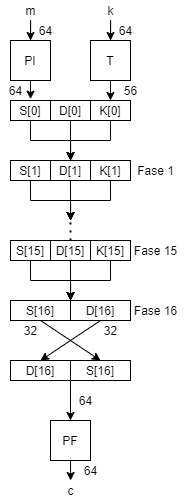
\includegraphics[width = 100pt]{images/DES_1.png}
\end{center} 
Nel grafico individuiamo:
\begin{itemize}
	\item m: blocco del messaggio (abbiamo in ingresso il blocco a 64 bit da criptare)
	\item k: chiave segreta con i bit di parità (64 bit, di cui 8 bit di parità)
	\item PI e PF: permutazione iniziale e finale (non ci sono sempre)
	\item c: corrispondente blocco del crittogramma (risultato finale dopo la $16-$esima fase)
\end{itemize}
Abbiamo in ingresso il messaggio $m$ a 64 bit e la chiave a 64 bit (di cui otto di parità). Permutiamo i bit del messaggio con $PI$, permutiamo anche i bit della chiave con $T$ ottenendo $K[0]$ Attenzione: $T$ restituisce solo 56 bit perchè scarta i bit di parità (di cui si conosce la posizione). A questo punto dividiamo il messaggio $m$ permutato (eventualmente permutato) in due blocchi: $S[0]$, $D[0]$. Eseguiamo una serie di fasi e alla fine, dopo l'ultima, scambiamo di posizione i blocchi $S[16]$ e $D[16]$. Eventualmente permutiamo.



\paragraph{Funzioni} In ogni fase $i=1,2,\dots,16$ andiamo ad applicare le seguenti funzioni:
\begin{align*}
	\text{S}[i] &= \text{D}[i-1]\\
	\text{D}[i] &= \text{S}[i-1] \oplus f\left(\text{D}[i-1],\text{K}[i-1]\right)
\end{align*}
Si scambiano le due metà dell'input, e D viene ottenuto con l'operatore XOR bit a bit tra $\text{S}[i-1]$ e una funzione non lineare $f\left(\text{D}[i-1],\text{K}[i-1]\right)$ (la S-box detta prima). Con le permutazioni e gli scambio realizzo la \textbf{diffusione} (lo vediamo perchè alterando un solo bit del messaggio in chiaro si ha un drastico cambiamento nell'intero crittogramma), con la S-box la \textbf{confusione} (la S-box prende in ingresso la chiave).

\paragraph{PI, PF e T} PI, PF e T sono delle tabella che vanno lette per riga:
\begin{center}
	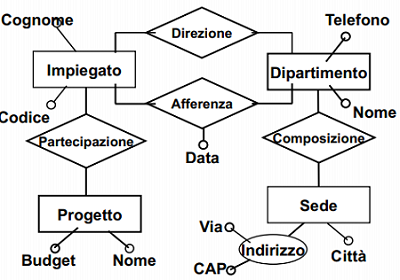
\includegraphics[scale=.5]{images/17.PNG}
\end{center}

\paragraph{Fase} La fase $i$-esima del DES è rappresentata dal seguente schema.
\begin{figure}[H]
    \centering
    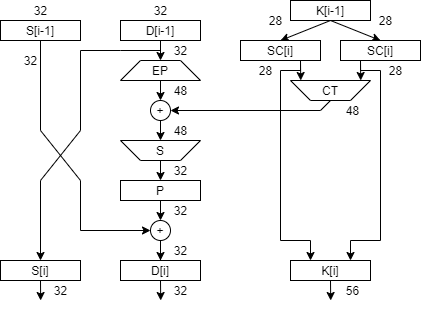
\includegraphics[width = 280pt]{images/DES_2.png}
\end{figure}
\noindent Abbiamo come input i blocchi $S[i-1]$, $D[i-1]$ (ottenuti dalla fase precedente, o i blocchi iniziali posti come indicato prima) e $K[i-1]$ (la chiave, alterata ad ogni step). La chiave viene divisa in due metà da 28 bit ciascuno. Su ciascuna metà si esegue uno shift ciclico (SC) a sinistra, dove il numero di posizioni dipende dall'indice della fase:
\begin{itemize}
	\item 1 se $i \in \{1, 2, 9, 16\}$
	\item 2 altrimenti
\end{itemize}
A questo punto i blocchi ottenuti vengono usati in due modi:
\begin{itemize}
	\item concatenati e posti come $K[i]$ (chiave usata nel prossimo step)
	\item concatenati e posti in ingresso in $CT$.
\end{itemize}
Il blocco CT permuta e scarta alcuni bit (si passa da 56 a 48 bit).Per quanto riguarda le due sequenze da 32 bit ($S[i-1]$ e $D[i-1]$):
\begin{itemize}
	\item pongo in $S[i]$ il contenuto di $D[i-1]$
	$$\text{S}[i]=\text{D}[i-1]$$
	\item pongo i bit di $D[i-1]$ in ingresso ne blocco EP, che permuta i bit e li espande (duplicazione di alcuni bit, si passa da 32 bit a 48 bit);
	\item applico lo XOR alle due sequenze a 48 bit (quella ottenuta da EP e quella ottenuta da CT)
	\item applico la S-box (che garantisce la non linearità della funzione, si passa da 48 a 32 bit);
	\item permuto i 32 bit ottenuti dalla S-box e applico l'operatore XOR tra questi ed $S[i-1]$.
\end{itemize}

\paragraph{Funzioni CT ed EP}
\begin{center}
	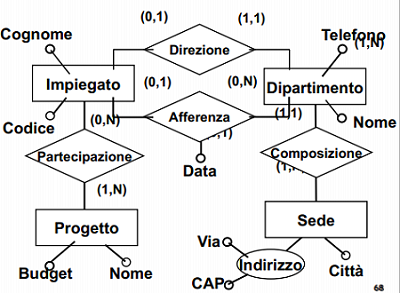
\includegraphics[scale=.5]{images/18.PNG}
\end{center}

\paragraph{S-Box} La S-box implementa 8 funzioni booleane a 6 input e a 4 output (in bit).
\begin{center}
    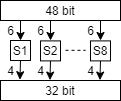
\includegraphics[width = 100pt]{images/DES_3.png}
\end{center}
Queste funzioni sono rappresentate attraverso delle tavola di verità, che vanno però lette in maniera particolare (di seguito la tabella di S1). Prendiamo il seguente esempio...
\begin{table}[ht!]
    \centering
    \small
    \begin{tabular}{c|c c c c c c c c c c c c c c c c}
        & 0 & 1 & 2 & 3 & 4 & 5 & 6 & 7 & 8 & 9 & 10 & 11 & 12 & 13 & 14 & 15 \\
        \hline
        0 & 14 & 4 & 13 & 1 & 2 & 15 & 11 & 8 & 3 & 10 & 6 & 12 & 5 & 9 & 0 & 7 \\
        1 & 0 & 15 & 7 & 4 & 14 & 2 & 13 & 1 & 10 & 6 & 12 & 11 & 9 & 5 & 3 & 8 \\
        2 & 4 & 1 & 14 & 8 & 13 & 6 & 2 & 11 & 15 & 12 & 9 & 7 & 3 & 10 & 5 & 0 \\
        3 & 15 & 12 & 8 & 2 & 4 & 9 & 1 & 7 & 5 & 11 & 3 & 14 & 10 & 0 & 6 & 13 \\
    \end{tabular}
\end{table}

\noindent Supponiamo di avere 010011: prendo gli estremi 0 ed 1 ed uso questo come indice per la riga, prendo poi i 4 bit centrali (1001) e lo uso come indice di colonna. Accedo quindi a (1, 9) $\xrightarrow{} 06$.

\paragraph{Perché è importante che non sia lineare?} Perché $$f(x \oplus y) \neq f(x) \oplus f(y)$$ ed è cruciale ai fini del funzionamento!

\section{Proprietà del DES con $m,c$ complementati}
Consideriamo i crittogrammi $c$, $c^{*}$, con il messaggio $m$ e la chiave $k$:
\begin{align*}
	c &= C_{DES}(m, k)&	c^{*} &= C_{DES}(\overline{m}, \overline{k})
\end{align*}
Abbiamo visto che prima della S-box applichiamo l'operatore XOR (ricordarsi $x \oplus 1=\overline{x}$)
$$ \bar{m_i} \oplus \bar{K_i} = (1 \oplus m_i) \oplus (1 \oplus K_i) = m_i \oplus K_i $$
Date le coppie $<m,k>, <\overline{m},\overline{k}>$ l'input della S-box \textbf{\underline{è lo stesso}}, dunque dalla S-box esce lo stesso output. In realtà il crittogramma restituito è il complemento
$$c^{*}=\overline{c}$$
Questo perchè nello XOR finale si ha complementazione in uno solo dei due blocchi (abbiamo un blocco posto direttamente che può essere complementato o no e un altro da cui otteniamo la stessa sequenza - \textit{S-box} - indipendentemente dall'essere complementato o no).
\paragraph{Esempio}
\begin{center}
	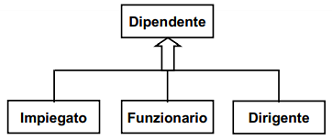
\includegraphics[scale=.75]{images/21.PNG}
\end{center}
\[\boxed{\text{\url{https://fauzanakmalh1.github.io/Simplified-DES-Calculator/}}}\]

\section{Attacchi al DES}
Gli attacchi al DES sono tutti attacchi a forza bruta:
\begin{itemize}
    \item \textbf{architetture appositamente progettate per attaccare il DES} e quindi velocizzare criptazione e decriptazione (con 1M\$ si costruiva una macchina che forzava il DES in 35 minuti);
    \item \textbf{distribuire lo spazio delle chiavi tra più utenti}, è più economico e la velocità dipende da quanti utenti vengono coinvolto.
\end{itemize}
\paragraph{\emph{challenges} di RSA} Nel 1997 la compagnia RSA ha offerto una ricompensa di diecimila dollari a chi avrebbe decifrato un crittogramma (non tanto trovare il messaggio, ma la chiave che ha prodotto quel particolare crittogramma attraverso il DES): in 5 mesi esplorando il 25\% delle chiavi viene risolta la sfida e trovata la chiave. Nel 1998 è stata lanciata una seconda sfida: ci vollero 39 di giorni esplorando 85\% delle chiavi.
\begin{align*}
	1997:\,\,&\text{strong cryptography makes the world a safer place}\\1998:\,\,&\text{many hands make light work}
\end{align*}

\subsection{Attacchi esaurienti} Le chiavi possibili sono $2^{56}$, 64 di queste chiavi sono rimosse perché con regolarità. Ricordando che:
\begin{align*}\boxed{C(m, k) = c}&&\boxed{\bar{c} = C(\bar{m}, \bar{k})}\end{align*}
si possono dimezzare le chiavi passando da $2^{56}$ a $2^{55}$ ($2^{56}=2\cdot 2^{55}$, 55 bit di sicurezza). Questo è un tipo di \textbf{attacco chosen plain-text} (scelto perchè i messaggi in chiaro devono avere una certa relazione) in cui il crittoanalista si procura delle coppie $$<m, c_1>, <\bar{m}, c_2>$$ Si inizia ad esplorare le chiavi e per ognuna si controlla:
\begin{itemize}
    \item $C(m, k) = c_1$: k probabilmente è la chiave
    \item $C(m, k) = \bar{c_2}$: $\bar{k}$ probabilmente è la chiave
    \item Se $c_1 \neq \bar{c_2}$ si prova un'altra chiave (k e $\bar{k}$ non lo sono)    
\end{itemize}
Possiamo dire
$$C(m,k) = \bar{c_2} \iff C(\bar{m},\bar{k}) = \bar{\bar{c_2}} = c_2$$
Escludo quindi due chiavi alla volta ($C(m,k)$ si calcola una volta soltanto, mentre la complementazione è operazione "tranquilla").

\subsection{Crittoanalisi differenziale} Nel 1990 sono stati scoperti attacchi di \emph{crittoanalisi differenziale} (da Bihan e Shamir).
\begin{itemize}
	\item E' un attacco di tipo \textbf{chosen plain-text} in cui il crittoanalista si procura $2^{47}$ coppie $<m,c>$ (messaggio scelto dal crittoanalista, obv).
	\item I messaggi sono scelti in modo tale da avere differenze particolari, il crittoanalista va a verificare le variazioni nel crittogramma. Si sfruttano le similitudini per arrivare alla chiave.
	\item Si assegnano delle probabilità alle singole chiavi, ed emerge poi quella più probabile.
\end{itemize}
\paragraph{Costo} Dato che le fasi sono 16 si ha un costo di questo attacco pari a $2^{55.1}$, poco più di una ricerca esaustiva (quindi nulla di interessante sul piano pratico). Con un numero di fasi minori, per esempio $8$, il costo si riduce drasticamente e allora il costo è minore rispetto alla ricerca esaustiva.

\subsection{Crittoanalisi lineare} Nel 1993 sono stati scoperti attacchi di \emph{crittoanalisi lineare} che consistono nella costruzione di una \underline{approssimazione lineare} della S-box che permette di inferire taluni bit della chiave, il resto si \textit{bruta}.
\paragraph{Costo} Si scende a $2^{43}$ coppie $<m, c>$ ed è di tipo known plain-text. Metodo più efficiente del forza bruta.

\section{Varianti del DES}
Il DES è sensibile agli attacchi di crittoanalisi differenziale e lineare, per renderlo più robusto si sono introdotte delle varianti. 
\subsection{Scelta indipendente delle sottochiavi}
Anziché generare le sottochiavi di fase a partire dalla chiave principale si scelgono manualmente.
E' come passare da 56 bit a $16 \cdot 48 = 768$ bit di chiave. \paragraph{Problema risolto?} Non abbiamo un effettivo aumento della sicurezza perché è sempre vulnerabile ad attacchi differenziali: si passa da 768 bit di sicurezza a 61 bit ($2^{61}$ la complessità).

\subsection{Cifratura multipla: 2DES}
Questa variante ha avuto maggiore successo rispetto alla precedente. L'idea è di applicare due volte la cifratura, di comporre il DES con se stesso:
$$ \forall k_1, k_2, k_3: C_D(C_D(m, k_1), k_2) \neq C_D(m, k_3) $$
applicare due volte la cifratura DES non è uguale ad applicarlo una sola volta.
Si arriva ad uno spazio delle chiavi di $2^{112}$.
\paragraph{Problema risolto?} L'attacco \emph{meet-in-the-middle} fa scendere la sicurezza a 57 bit di sicurezza:
$$ c = C(C(m,k_1), k_2) $$
facciamo la decifrazione di $C$ con la chiave $k_2$ (tolgo la cifratura più esterna)
$$ D(c,k_2) = C(m,k_1) $$
possiamo quindi prendere una coppia $<m, c>$:
\begin{itemize}
	\item $ \forall k_1 \text{ calcolo e salvo } C(m, k_1) \xrightarrow{} 2^{56} \text{ cifrature (tutte)}$
	\item $ \forall k_2 \text{ calcolo e verifico corrispondenza di } D(c, k_2) \xrightarrow{} 2^{56} \text{ cifrature (al più) }$
\end{itemize}
Cercando nella lista delle cifrature, so che esisterà una coppia $<k_1, k_2>$ per la quale c'è la corrispondenza:
$$ D(c, \bar{k_2}) = C(m, \bar{k_1}) $$
Questo attacco costa quindi $2^{56} + 2^{56} = 2 \cdot 2^{56} = 2^{57}$ al più, tra cifrature e decifrature. Cioè l'aumento di complessità dovuto alla doppia cifratura non è di $N^2$ ma di $2N$
$$2N << N^2$$


\subsection{Cifratura multipla: 3DES}
Nella pratica non si è fatta una doppia cifratura. 
\begin{itemize}
    \item \textbf{2TDEA} (proposta a due chiavi):
        $$ c = C\left(D(C(m, k_1), k_2), k_1\right) $$
        $k_1$ e $k_2$ sono chiavi di 56 bit tra di loro indipendenti. Si sceglie questa modalità (CDC invece di CCC) per mantenere la compatibilità abilitati a usare un singolo DES. Se pongo $k_1 = k_2$ ottengo il DES normale (cifratura singola).
        
        {Attenzione}: CDC non è più robusto di CCC. Un attacco \emph{meet-in-the-middle} ha un costo di 112 bit.
    \item \textbf{3TDEA} (\textit{triple data encryption algorithm}):
        $$ c = C(D(C(m, k_1), k_2), k_3) $$
        $k_1$, $k_2$, $k_3$ sono chiavi a 56 bit. Si hanno chiavi di $3 \cdot 56 = 168$ bit. In realtà è vulnerabile ad attacchi \textit{meet-in-the-middle} quindi la sicurezza scende da 168 bit a 112 bit di sicurezza.
        
        Per ottenere il messaggio decifriamo usando le chiavi in ordine inverso
        $$m=D\left(C(D(c,k_3),k_2),k_1\right)$$
        Osserviamo banalmente che
        $$C(m,k_1)=C(D(c,k_3),k_2)$$
        come prima 
        $$\forall k_1 \text{ calcolo e salvo } C(m,k_1)$$
        successivamente
        $$\forall k_2,k_3 \text{ calcolo } C(D(c,k_3),k_2) \text{ e lo cerco nella lista}$$
        A livello di costo otteniamo $O\left(2^{56}+2^{112}\right)=O\left(2^{112}\right)$.
\end{itemize}

